\documentclass[final,1p,times]{elsarticle}

\usepackage{amsmath,amssymb}
\usepackage{booktabs}
\usepackage{siunitx}
\usepackage{adjustbox}
\usepackage{float}
\usepackage{hyperref}

\journal{Applied Thermal Engineering}
\bibliographystyle{elsarticle-num}

\begin{document}

\begin{frontmatter}

\title{Coupled Thermal and Acoustic Characterization of Energy Storage-Release Dynamics in Microbubble Emission Boiling}

\author[inst1]{Mohamamd Ishraq Hossain}
\author[inst1]{Stephen Pierson}
\author[inst1]{Han Hu}
\affiliation[inst1]{organization={Department of Mechanical Engineering, University of Arkansas}, city={Fayetteville}, state={AR}, postcode={72701}, country={USA}}
% \cortext[cor1]{Corresponding author.}
% \ead{corresponding.author@example.edu}

\begin{abstract}
Microbubble emission boiling (MEB) can remove heat fluxes beyond conventional pool-boiling limits, but its onset and development remain difficult to diagnose because wall heat transfer, vapor collapse, liquid replenishment, and acoustic emission evolve together. This study develops a time-resolved thermal-acoustic workflow for subcooled pool boiling on a flat copper surface and applies it to four tests near 97-98 kPa with power levels from 150 to 250 W. Wall temperature and heat flux are reconstructed from embedded thermocouple data. Hydrophone signals are reduced to spectrograms, band-integrated voltage-PSD power proxies, and characteristic frequencies; acoustic-emission waveform analysis is performed for the two cases with available waveform files. Maximum reconstructed heat flux increases from 142 to 278 W/cm$^2$ across the power sweep. Two high-power cases exhibit post-transition thermal and acoustic oscillations, whereas lower-power cases do not show that developed state. Event markers separate the transition-associated heat-flux drop, wall-temperature peak, first sustained oscillation peak, and power shutoff. In the developed cases, hydrophone and acoustic-emission data show slow envelope modulation near 0.05 and 0.08 Hz, describing regime-scale modulation rather than bubble-collapse carrier frequencies. Hilbert-envelope analysis shows rapid thermal-envelope saturation in one developed case and slower growth in the highest-power case. Representative video frames support a storage-release interpretation in which near-wall vapor/thermal energy accumulates before intermittent microbubble release. Calibration-limited uncertainty estimates are reported for the main thermal and acoustic metrics. The results position synchronized thermal-acoustic diagnostics as a route for identifying MEB development and distinguishing slow regime modulation from high-frequency collapse signatures.
\end{abstract}

\begin{keyword}
microbubble emission boiling \sep subcooled pool boiling \sep boiling sound \sep hydrophone \sep acoustic emission \sep heat flux \sep oscillation envelope
\end{keyword}

\begin{highlights}
\item Thermal-acoustic diagnostics identify developed microbubble emission boiling.
\item Hydrophone data separate slow regime modulation from collapse-frequency content.
\item Acoustic-emission waveforms confirm high-power modulation through a second path.
\item Envelope fits quantify growth and saturation of thermal oscillations.
\item Video frames support a vapor/thermal storage-release mechanism.
\end{highlights}


\end{frontmatter}

\section*{Nomenclature}
\begin{center}
\small
\begin{tabular}{@{}p{0.16\textwidth}p{0.56\textwidth}p{0.16\textwidth}@{}}
\toprule
    Symbol & Definition & Unit \\
\midrule
    $A$ & oscillation envelope amplitude & signal-dependent \\
    $A_0$ & fitted envelope amplitude at the first sustained oscillation peak & signal-dependent \\
    $A_\infty$ & fitted asymptotic envelope amplitude & signal-dependent \\
    $C_{\mathrm{eff}}$ & effective thermal/vapor storage capacitance in reduced-order model & J/K or normalized \\
    \texttt{E\_stored} & stored near-wall thermal/vapor energy per unit area & J/cm\textasciicircum{}2 or normalized \\
    $f$ & frequency & Hz \\
    $H$ & Heaviside-like release switch in reduced-order model & dimensionless \\
    $K_{\mathrm{eff}}$ & effective nonlinear restoring coefficient in reduced-order model & normalized \\
    $L_{\mathrm{eff}}$ & effective inertial element for vapor-film/liquid response & normalized \\
    $P_{\mathrm{load}}$ & electrical power load & W \\
    $\Phi$ & nonlinear feedback term in reduced-order model & normalized \\
    $q''$ & heat flux & W/cm$^2$ \\
    \texttt{q''\_in} & heat-flux input to the near-wall storage volume & W/cm$^2$ \\
    \texttt{q''\_loss} & heat-flux loss during storage between release bursts & W/cm$^2$ \\
    \texttt{q''\_release} & transient release heat-flux contribution during vapor collapse or rewetting & W/cm$^2$ \\
    $T$ & temperature & °C \\
    $T_{\mathrm{sat}}$ & saturation temperature & °C \\
    $T_w$ & extrapolated wall temperature & °C \\
    $t_{\mathrm{DNB}}$ & transition-associated heat-flux maximum before the sudden drop & s \\
    $t_{\mathrm{off}}$ & time when DC power is turned off & s \\
    $t_{\mathrm{osc}}$ & first sustained wall-temperature oscillation peak in the analysis window & s \\
    $t_{\mathrm{peak}}$ & wall-temperature peak during the transition event & s \\
    $\tau$ & asymptotic envelope growth time constant & s \\
    $\Theta$ & normalized stored-state variable in reduced-order model & dimensionless \\
    $\xi$ & normalized release-coordinate variable in reduced-order model & dimensionless \\
\bottomrule
\end{tabular}
\end{center}
\normalsize

\section{Introduction}

Boiling heat transfer is attractive because phase change can remove heat fluxes far beyond those accessible to single-phase convection. Its practical use, however, is constrained by boiling crisis: vapor accumulation near the wall can interrupt liquid contact, reduce heat-transfer effectiveness, and produce rapid wall-temperature excursions. Classical hydrodynamic treatments of critical heat flux (CHF), including the work of Zuber \citep{zuber_1958_stability,zuber_1959_hydrodynamic}, established the importance of vapor-liquid interfacial instability, and later texts and reviews organized CHF mechanisms, correlations, and subcooling effects for engineering design \citep{carey_2020_phase_change,liang_2018_chf_review}. These foundations remain essential, but they do not fully describe regimes in highly subcooled liquids where condensation, vapor collapse, liquid replenishment, and acoustic emission evolve together after departure from ordinary nucleate boiling.

Microbubble emission boiling (MEB) sits in this unsettled part of the boiling map. Early subcooled-boiling observations showed that strong subcooling changes bubble growth and collapse \citep{gunther_1950_subcooled_bubble_photography,ivey_1966_subcooled_chf}, and subsequent studies identified the emission of fine bubbles from near-wall vapor structures as a distinct high-heat-flux behavior \citep{inada_1981_subcooled_pool_boiling,zeigarnik_2012_microbubble_emission_nature}. The important point is not only that MEB can be associated with large heat fluxes. It is that MEB appears to operate through a coupled cycle: vapor structures form or coalesce, collapse rapidly in subcooled liquid, emit microbubbles and sound, and drive liquid motion back toward the wall. Visualized MEB experiments, transition studies, and spatiotemporal surface-temperature measurements support this interpretation by showing rapid vapor collapse, nonuniform surface-temperature fields, and boiling-sound signatures during MEB development \citep{zhu_2014_visualized_meb,tang_2016_transition_to_meb,tang_2019_transient_nucleate_to_meb,horiuchi_2021_spatial_temporal_thermal_fluid}. Recent measurements that connect bubble-induced oscillating flow and vapor-film motion to heat transfer further suggest that MEB should be treated as a coupled thermal-fluid oscillatory regime rather than only as a point on a boiling curve \citep{li_2022_oscillating_vapor_film,tang_2023_bubble_induced_oscillating_flow}.

That physical picture creates an important diagnostics problem. If the key process is coupled and unsteady, then a boiling curve alone cannot tell whether a case is entering MEB, whether the oscillatory state is strengthening, whether heating and cooling follow a hysteretic path after power shutoff, or whether acoustic activity is synchronized with wall-temperature and heat-flux changes. Yet many available comparisons emphasize heat flux, onset wall superheat, visualization snapshots, or acoustic classification separately. Surface-condition studies show that MEB onset depends on surface properties as well as heat flux and subcooling \citep{unno_2022_surface_properties_meb_onset}, and reduced-pressure or confined-vessel studies indicate that onset can shift under conditions relevant to subatmospheric operation \citep{unno_2025_reduced_pressure_confined_meb}. Specialized configurations such as cavitation-assisted boiling, open microchannels, and engineered surfaces demonstrate the breadth of MEB-like heat-transfer behavior but also make clear that geometry, confinement, pressure, surface preparation, and regime definition must be preserved before literature heat-flux values can be compared meaningfully \citep{inada_2016_cavitation_bubble_blow_pit,zhao_2025_open_microchannel_meb,elele_2018_single_bubble_boiling,liu_2020_pin_cluster_nucleation}. The missing need is not another isolated heat-flux number; it is a time-resolved way to connect thermal response, acoustic response, event timing, and MEB-state development in one record.

Acoustic measurements are a natural candidate for that role because MEB is often loud, intermittent, and collapse-driven. Sound-emission studies in subcooled pool boiling have reported spectral features associated with MEB \citep{tang_2018_sound_emission_subcooled_pool}, and hydrophone-based acoustic state detection has shown that boiling sound can classify MEB states \citep{ono_2023_acoustic_state_detection_meb,ueki_2024_acoustic_state_cucrzr_divertor}. Broader boiling-crisis studies have also used audio-visual-thermal measurements and deep-learning classifiers to identify regime transitions \citep{sinha_2020_audio_visual_thermal_transition,sinha_2021_deep_learning_sound_boiling}, while AE monitoring has demonstrated that boiling-induced elastic waves can carry regime information through a heated structure \citep{baek_2017_ae_water_boiling_cladding}. These results show that acoustic signals contain useful information, but they also expose a trap: a single reported frequency can mean very different things. Bubble-collapse or boiling-sound carrier frequencies may lie from tens of Hz to several kHz \citep{tang_2016_transition_to_meb,zhu_2014_visualized_meb,horiuchi_2021_spatial_temporal_thermal_fluid,kobayashi_2022_on_homogeneity_of_vapor_bubble}, whereas band-integrated acoustic-amplitude proxies can oscillate much more slowly as the boiling state grows, saturates, or intermittently bursts. Without synchronized thermal data, these frequency scales can be confused.

The present study addresses that gap by developing a reproducible thermal-acoustic workflow for subcooled pool boiling on a flat copper surface. Four active-heating cases are analyzed in order of increasing imposed electrical power and are referred to as Cases A-D rather than by internal test identifiers. Wall temperature and heat flux are reconstructed from embedded thermocouples for all four cases. Hydrophone signals are reduced to spectrograms, band-integrated voltage-PSD power proxies, and characteristic frequencies for all four cases. AE waveform analysis is included only for Cases C and D, because those are the cases with available waveform files. The analysis defines event times for the transition-associated heat-flux drop, the wall-temperature peak during transition, the first sustained oscillation peak, and power shutoff. It then uses these events to compare heating-only boiling curves, aligned thermal-acoustic time histories, slow acoustic modulation, and asymptotic growth of oscillation envelopes. The goal is not to establish a universal MEB onset correlation from four tests. Rather, it is to show how synchronized thermal, hydrophone, AE, and video diagnostics can distinguish lower-power reference behavior from a developed oscillatory MEB-like state and can prevent confusion between slow regime modulation and high-frequency collapse signatures. A source-status-labeled MEB literature compilation is used not as a stand-alone review, but as context for two questions that remain unresolved: how MEB onset and heat-transfer scale should be compared across very different experiments, and how acoustic frequencies should be interpreted when carrier, bubble-cycle, and slow-envelope scales coexist.

\section{Experimental Data and Analysis Workflow}

The experimental dataset consists of four subcooled pool-boiling tests on a flat copper surface. The cases were conducted near 97-98 kPa with water as the working fluid. The imposed electrical power was increased across the matrix from approximately 150 W to 250 W. Table 1 summarizes the operating conditions and primary thermal outcomes. The values come from the reproducible BoilingLab multi-case analysis, which retains only the active-heating portion of each test.

The experiments were performed in a pressure-controlled stainless-steel pool-boiling chamber with optical access through reinforced glass viewports. The chamber was fitted with a reflux condenser and an internal coiled condenser loop connected to a temperature-controlled chiller so that vapor generation during boiling could be balanced by condensation. Pressure was adjusted with a vacuum pump and condenser-flow control, while the bulk liquid and vapor-space temperatures were monitored with T-type thermocouples. A dedicated facility paper will describe the chamber, pressure-control approach, and operating procedure in detail; only the elements needed to interpret the present thermal-acoustic data are summarized here.

The heated specimen was mounted in a heating-element enclosure inserted through the chamber base. For the cases considered here, the boiling surface was a flat, upward-facing copper surface with a projected area of 10 mm by 10 mm. Four T-type thermocouples were embedded along the copper centerline below the surface at uniform axial spacing. Their temperatures were used to estimate the wall temperature and heat flux by a one-dimensional conduction model. Electrical heat input was supplied by cartridge heaters powered by a programmable DC power supply, and the power-supply voltage, current, and power were logged during each test.

\begin{table}[t]
  \centering
  \caption{Summary of active-heating cases used in this draft.}
  \resizebox{\textwidth}{!}{%
  \begin{tabular}{lcccccc}
    \toprule
    Case & Nominal power (W) & Mean pressure (kPa) & Mean liquid temperature (°C) & $T_{\mathrm{sat}}$ (°C) & Maximum $q''$ (W/cm$^2$) & Maximum $T_w$ (°C) \\
    \midrule
    A & 150 & 97.28 & 58.83 & 98.84 & 142.0 & 112.7 \\
    B & 180 & 97.30 & 52.38 & 98.84 & 163.1 & 159.2 \\
    C & 230 & 97.47 & 57.27 & 98.89 & 267.2 & 167.0 \\
    D & 250 & 97.51 & 57.60 & 98.90 & 278.0 & 172.9 \\
    \bottomrule
  \end{tabular}
  }
\end{table}

The dataset is intentionally interpreted as a pilot study. Cases A and B provide lower-power references. Cases C and D contain the strongest evidence of developed coupled thermal-acoustic oscillations and have the most complete acoustic analysis, including hydrophone and AE waveform processing. Thermal data are available for all four cases; AE waveform files are available only for Cases C and D. The limited number of tests does not support a universal MEB scaling law, but it is sufficient to demonstrate a synchronized analysis method and to identify physically meaningful differences between lower- and higher-power responses.

\begin{table}[t]
  \centering
  \caption{Data coverage and interpretation scope for each case.}
  \resizebox{\textwidth}{!}{%
  \begin{tabular}{lcccccc}
    \toprule
    Case & Nominal power (W) & Thermal reconstruction & Hydrophone diagnostics & AE waveform diagnostics & High-speed video frames & Interpretation scope \\
    \midrule
    A & 150 & yes & yes & no waveform file & available & lower-power reference \\
    B & 180 & yes & yes & no waveform file & available & lower-power reference \\
    C & 230 & yes & yes & yes & available & developed oscillatory MEB-like case \\
    D & 250 & yes & yes & yes & available & developed oscillatory MEB-like case \\
    \bottomrule
  \end{tabular}
  }
\end{table}

The phrase "developed oscillatory MEB-like case" is used in a diagnostic sense rather than as a universal regime boundary. The assignment follows the signatures emphasized in MEB literature: fine microbubble emission from near-wall vapor structures, rapid vapor collapse in subcooled liquid, high heat flux, boiling-sound or acoustic activity, and oscillatory vapor/thermal behavior. A case is assigned to this group only when four criteria are satisfied together in the present measurements: a resolved transition-associated heat-flux maximum, sustained post-transition wall-temperature and heat-flux oscillations, hydrophone band-power modulation in the same active-heating interval, and visual evidence of intermittent microbubble release. Table 3 makes this classification auditable. A low-frequency component extracted from a lower-power hydrophone record is therefore not interpreted as an MEB modulation frequency unless the thermal and visual criteria are also met.

\begin{table}[t]
  \centering
  \caption{Operational criteria used to classify developed oscillatory MEB-like behavior.}
  \resizebox{\textwidth}{!}{%
  \begin{tabular}{lcccccc}
    \toprule
    Case & Power (W) & Transition marker & Thermal oscillation & Acoustic modulation & Video support & Classification \\
    \midrule
    A & 150 & no & no & hydrophone available, no MEB interpretation & no sustained-release frame set assigned & lower-power reference \\
    B & 180 & yes & no sustained post-transition oscillation & hydrophone available, no MEB interpretation & no sustained-release frame set assigned & lower-power reference \\
    C & 230 & yes; \texttt{t\_DNB = 150.8 s} & yes; \texttt{t\_osc = 321.6 s} & 0.050 Hz hydrophone; 0.055 Hz AE & screened frames support intermittent release & developed oscillatory MEB-like case \\
    D & 250 & yes; \texttt{t\_DNB = 124.8 s} & yes; \texttt{t\_osc = 308.0 s} & 0.080 Hz hydrophone; 0.080 Hz AE & screened frames support intermittent release & developed oscillatory MEB-like case \\
    \bottomrule
  \end{tabular}
  }
\end{table}

Thermal quantities are reconstructed from the embedded thermocouple array. Temperatures are read from LVM files and used to reconstruct the surface temperature by extrapolating embedded thermocouple measurements through the copper block. Heat flux is calculated from the inferred temperature gradient and the copper thermal conductivity. The approach assumes one-dimensional conduction over the thermocouple line used for extrapolation. The quality of the linear fit through the thermocouple data is stored in the generated summaries and provides a check on the conduction approximation.

The multi-case boiling curves include only heating data. Samples are retained when the aligned DC-power signal is positive. This definition removes the cooling path after power shutoff, which would otherwise mix active boiling behavior with post-heating thermal relaxation. It also makes the comparison more consistent with literature boiling curves that represent increasing or active heat input.

Event times define the analysis windows. Four event times are extracted from each developed case. The transition-associated time $t_{\mathrm{DNB}}$ is defined operationally as the heat-flux maximum before the sudden heat-flux drop during transition. The symbol is retained because the event resembles the departure-from-nucleate-boiling or vapor-coverage marker used in boiling practice, but the present measurements do not by themselves prove a classical DNB mechanism. The wall-temperature peak $t_{\mathrm{peak}}$ identifies the thermal overshoot during that transition. The first sustained oscillation marker $t_{\mathrm{osc}}$ is extracted from the first wall-temperature oscillation peak after the nominal start of the oscillatory window. It is not treated as a universal MEB onset time; it defines the start of the envelope-analysis interval for the developed oscillatory state. The shutoff time $t_{\mathrm{off}}$ is defined from the DC-power signal when the power load returns to near zero.

These definitions intentionally separate transition and sustained oscillation. The heat-flux drop and wall-temperature peak occur early in the record and describe the departure from the preceding boiling path. The later $t_{\mathrm{osc}}$ marker defines the start of the envelope-analysis interval for the sustained MEB-like oscillatory state. Event-time uncertainty is treated as an expanded \texttt{k = 2} allowance of 1.0 s, combining wall-clock synchronization, sampled time-bin width, and event-picking sensitivity.

Acoustic sensing is treated as a synchronized but sensor-dependent diagnostic. Two acoustic pathways were used. A High-Tech HTI-96-MIN hydrophone was immersed in the liquid pool to sense pressure fluctuations and boiling sound transmitted through the working fluid. The hydrophone signal was acquired with a National Instruments NI-9230 module using LabVIEW. A MISTRAS R3a acoustic-emission sensor was mounted on the outside wall of the stainless-steel chamber to sense structure-borne acoustic activity generated by boiling and transmitted through the vessel. The AE sensor was connected to a MISTRAS EasyAE system and recorded with AEWin software. The thermal, power, hydrophone, and AE records were synchronized through wall-clock time stamps before post-processing in BoilingLab.

Hydrophone data are analyzed with spectrograms and PSD-based band integration. The hydrophone spectrogram uses a Hann-windowed short-time Fourier transform with 8192 samples per segment and 50\% overlap. Band-integrated hydrophone power is obtained by integrating the voltage PSD over 0-6 kHz in linear units before any logarithmic display. This band was chosen because the displayed hydrophone spectrograms and characteristic-frequency histories concentrate the repeatable boiling-sound content in the low-kilohertz range, while avoiding higher-frequency regions that were not used consistently across the hydrophone figures. The result is a voltage-squared band-power proxy, not a calibrated acoustic intensity. Direct averaging of dB values is avoided because dB is logarithmic and does not preserve linear acoustic power. The publication-analysis tables record the current data coverage explicitly: generated hydrophone intermediates are available for all four cases, while AE waveform files are available only for Cases C and D. A band-sensitivity check was also performed for the two developed cases by repeating the band integration over 0-3, 0-6, and 0-10 kHz. The dominant slow modulation frequency was unchanged across these three bands within each case: 0.055 Hz for Case C and 0.075 Hz for Case D in the sensitivity calculation.

Characteristic acoustic frequencies are extracted from each spectrogram time bin. The peak frequency identifies the largest PSD bin in the selected band. The spectral centroid gives the power-weighted frequency, and the bandwidth measures the spread around the centroid. These metrics are plotted over time and compared with the integrated voltage-PSD power proxy to determine whether amplitude bursts align with shifts in spectral content. The slow modulation frequency is then extracted from the band-integrated power-proxy trace over the active oscillatory window. The trace is mean-subtracted, linearly detrended, and analyzed with a Hann-window Welch PSD using 50\% segment overlap. The dominant frequency is selected as the largest PSD peak between the inverse window duration and 0.2 Hz. This procedure is applied to all hydrophone records, but the resulting value is interpreted as an MEB modulation only when the case also satisfies the thermal and visual criteria in Table 3.

AE waveform files are processed with the same overall logic for Cases C and D. The AE waveform spectrogram uses windowed FFT blocks based on the waveform record length, and the default AE PSD integration band is 0-250 kHz. The AE sensor responds through a different transmission path than the hydrophone, so agreement between hydrophone and AE modulation is meaningful. It indicates that the slow oscillatory behavior is not an artifact of one sensor alone. Because the AE sensor is mounted on the chamber wall rather than immersed in the liquid, AE power is interpreted as a structure-path-weighted voltage proxy rather than an absolute acoustic intensity.

The oscillation-amplitude analysis uses a Hilbert-transform envelope. For each signal, the active MEB window is selected, a slow baseline is removed using a 75 s Savitzky-Golay smoother, and the Hilbert envelope of the detrended signal is smoothed with a 35 s Savitzky-Golay window. The smoothed envelope is fitted with a first-order asymptotic growth model:

\begin{equation}
A(t) = A_{\infty} - \left(A_{\infty} - A_0\right)\exp\left[-\frac{t-t_{\mathrm{osc}}}{\tau}\right].
\label{eq:envelope}
\end{equation}

Here $A_0$ is the fitted envelope amplitude at $t_{\mathrm{osc}}$, $A_\infty$ is the asymptotic envelope amplitude, and $\tau$ is the growth time constant. The fitted saturation fraction at the end of the window is \path{(A_end - A_0)/(A_inf - A_0)}. The model is not intended to prove a universal first-order process. It is used as a compact metric for whether the envelope continues to grow linearly, approaches a finite amplitude, or is poorly described by smooth saturation.

The literature comparison is maintained in the sibling \texttt{literature-compiler} repository under \path{examples/test2_meb}. The case includes MEB-related Zotero sources, screening notes, curated heat-flux and wall-superheat values, manually digitized boiling-curve traces from the available PDFs, and a separate table of MEB-specific acoustic and oscillatory signatures. The compilation is used in this manuscript as a structured context rather than as a finalized systematic review. Values marked as reported text or range endpoints require checking against the original figures and tables before cross-study scaling; values marked as figure digitized should be treated as approximate trace extractions until final WebPlotDigitizer-style calibration and uncertainty assignment are completed.

The compilation also records frequency type. This field is essential because the literature contains several different frequency quantities: bubble oscillation frequency, boiling sound peak frequency, pressure fluctuation frequency, hydrophone sampling rate, and slow envelope modulation. The present work reports slow envelope modulation of thermal response and acoustic voltage-PSD proxies, so comparisons to high-frequency sound or bubble-collapse values must be made through mechanism rather than by direct numerical equality.

\section{Results and Discussion}

\subsection{Heating-only boiling curves identify the power range where the oscillatory state appears}

Figure 1 shows two complementary boiling-curve views. Figure 1a retains only the active-heating portions and is therefore the appropriate panel for comparing the increasing-power boiling response among cases. The heat flux increases with wall superheat during early heating and then separates by input power. Cases A and B reach maximum reconstructed heat fluxes of 142 and 163 W/cm$^2$, respectively. Cases C and D reach substantially higher values, 267 and 278 W/cm$^2$. These values are reconstructed from embedded thermocouple gradients over the 10 mm by 10 mm projected heater area and therefore represent filtered wall heat-flux estimates. The higher-power cases also show a different time-domain response, with persistent post-transition oscillations in wall temperature and heat flux.

Figure 1b includes the full thermal history and separates heating and cooling branches. This view is not used to define active boiling performance after power shutoff, but it is useful for identifying hysteresis. During heating, the high-power cases enter the developed oscillatory MEB-like state only after the transition event and subsequent growth of oscillations. During cooling, the curves do not retrace the same path. Once power is removed, near-wall vapor collapse, rewetting, liquid replenishment, and thermal relaxation occur while the copper block still contains stored energy. The return from the MEB-like state to nucleate boiling or single-phase cooldown therefore follows a different trajectory from the entry path. This hysteresis is physically consistent with a storage-release process: the vapor/liquid structure and solid thermal field have memory, so the local heat-flux estimate during cooling reflects both residual stored energy and the changing boiling state rather than only the instantaneous electrical input.

The figure has two roles in the manuscript. First, it establishes that the four tests are not identical repeats but a power sweep across lower- and higher-intensity boiling responses. Second, it shows why a boiling curve alone is insufficient for this dataset. Cases C and D are close in maximum heat flux, but their time-domain envelope metrics differ strongly. Case C approaches a saturated thermal oscillation amplitude more rapidly, while Case D continues to develop more slowly until power shutoff. That difference is invisible if the data are reduced only to maximum heat flux or a single curve envelope.

Physically, the progression from Cases A/B to Cases C/D is consistent with increasing vapor generation and stronger interaction between near-wall vapor structures and subcooled liquid. The higher-power cases likely provide enough vapor generation to sustain repeated vapor collapse and liquid replenishment, while the lower-power cases remain weaker or less organized. This interpretation agrees with literature that connects MEB to high subcooling, high heat flux, bubble collapse, and oscillating liquid motion \citep{zhu_2014_visualized_meb,tang_2016_transition_to_meb,tang_2023_bubble_induced_oscillating_flow}.

\begin{figure}[H]
  \centering
  
\includegraphics[width=\linewidth]{fig01_heating_boiling_curves.pdf}
  \caption{Boiling curves for the four cases. Panel (a) shows heating-only $q''$ versus wall superheat using samples with positive DC power. Panel (b) shows the full thermal history; solid lines are heating before power shutoff and dashed lines are cooling after shutoff. The corner marker gives the maximum expanded uncertainty ($k=2$) for $T_w$ and $q''$ among the four cases.}
  \label{fig:1}
\end{figure}

\subsection{Event markers distinguish transition from sustained oscillatory MEB-like behavior}

Figure 2 shows the high-power Case D time histories with event markers. The heat flux initially increases, reaches a local maximum before a sudden drop, and then recovers into a sustained oscillatory regime. The transition-associated $t_{\mathrm{DNB}}$ marker occurs at 124.8 s, and the wall-temperature peak occurs at 132.4 s. The first sustained oscillation peak used for envelope analysis occurs later at 308.0 s, while power is turned off at 673.9 s. The separation between these markers is important: the heat-flux maximum is a transition marker, whereas the later $t_{\mathrm{osc}}$ marker is a windowing marker for sustained oscillation.

This sequence indicates that the transition event and the sustained oscillatory state are separated in time. The early heat-flux drop and wall-temperature peak are consistent with a departure from a nucleate-boiling-like path and a transient vapor-coverage or dryout event. The later oscillatory interval is different: wall temperature and heat flux oscillate repeatedly while power remains on. This behavior is closer to the MEB descriptions in which vapor structures repeatedly grow, condense, collapse, and interact with the surrounding liquid.

Figure 3 shows the same analysis for Case C. It is retained because it adds information that Figure 2 alone cannot provide. Case D is the highest-power case and shows an earlier transition, whereas Case C is the lower-power developed case and tests whether the same event sequence appears under a different thermal forcing. In Case C, the transition-associated $t_{\mathrm{DNB}}$ marker occurs at 150.8 s, the wall-temperature peak occurs at 160.8 s, the first sustained oscillation peak occurs at 321.6 s, and power shutoff occurs at 757.8 s. Compared with Case D, Case C begins its sustained oscillatory interval slightly later but has a longer active-heating duration after $t_{\mathrm{osc}}$. This longer window partly explains why its thermal envelope approaches saturation more completely. Thus Figure 3 demonstrates that the developed oscillatory state is reproducible across the two high-power cases, while also showing that envelope growth and saturation are not controlled by nominal power alone.

The event markers make the analysis auditable. Without them, the envelope window could be chosen subjectively, and transition overshoot could be mixed with sustained oscillation. The markers also create a bridge to the literature. Prior MEB transition studies often focus on the abrupt transition or visual onset \citep{tang_2016_transition_to_meb,tang_2019_transient_nucleate_to_meb}, while acoustic state studies focus on regime classification \citep{ono_2023_acoustic_state_detection_meb}. The present marker set links those perspectives by defining both the transition and the later oscillatory state in one synchronized record. This distinction is also important for practical thermal-system monitoring: a sensor strategy that identifies only the transition event may miss whether the post-transition state stabilizes, strengthens, or remains intermittent under continued heating.

\begin{figure}[H]
  \centering
  
\includegraphics[width=\linewidth]{fig02_case_d_thermal_time_histories.pdf}
  \caption{Thermal time histories for the highest-power case. Panel (a) shows heat flux and power load versus time. Panel (b) shows embedded thermocouple temperatures and extrapolated wall temperature. Dashed vertical markers identify $t_{\mathrm{DNB}}$, $t_{\mathrm{peak}}$, $t_{\mathrm{osc}}$, and $t_{\mathrm{off}}$; $t_{\mathrm{DNB}}$ is used as an operational transition-associated heat-flux maximum.}
  \label{fig:2}
\end{figure}

\begin{figure}[H]
  \centering
  
\includegraphics[width=\linewidth]{fig03_case_c_thermal_time_histories.pdf}
  \caption{Thermal time histories for the second developed high-power case, plotted with the same definitions and event markers as Fig.~\ref{fig:2}.}
  \label{fig:3}
\end{figure}

\subsection{Hydrophone spectra and band-integrated power proxies show slow modulation of the developed regime}

Figure 4 shows the hydrophone diagnostics. The spectrogram identifies the frequency content of the acoustic signal, while the band-integrated voltage-PSD power proxy converts the PSD into a scalar relative metric over time. The characteristic-frequency plot shows how peak frequency and spectral centroid evolve during the same interval. Hydrophone metrics are now available for all four cases. Cases A and B provide lower-power acoustic references, while Cases C and D show stronger band-integrated hydrophone power proxies and clearer sustained oscillatory behavior during the developed MEB-like regime.

The lower-power cases do not show sustained MEB-like oscillations, so their mechanically extracted low-frequency components are not interpreted as MEB modulation frequencies. The developed high-power cases do show a repeatable slow modulation frequency of the band-integrated voltage-PSD proxy: approximately 0.05-0.055 Hz for Case C and 0.075-0.08 Hz for Case D, depending on the exact time-grid and Welch-bin resolution used in the summary and band-sensitivity calculations. AE waveform analysis gives nearly the same modulation values for the two developed high-power cases, approximately 0.055 Hz and 0.080 Hz. The agreement between hydrophone and AE modulation is important because the two sensors have different coupling paths. The hydrophone senses pressure waves in the liquid, whereas AE senses elastic/acoustic activity transmitted through the solid structure. Agreement between them suggests that the slow modulation in Cases C and D is a real boiling-state feature rather than a single-sensor artifact.

The hydrophone power-proxy and centroid-frequency traces are not independent in the developed cases. Normalized cross-correlation over the oscillatory window gives a best lag of approximately +0.64 s for Case C with a correlation coefficient of 0.82 and -0.64 s for Case D with a coefficient of 0.64. These lags are small compared with the 12.5-20 s modulation periods, indicating that acoustic-amplitude bursts and centroid-frequency changes are nearly synchronous at the slow-envelope scale. This supports the interpretation that the slow modulation is consistent with a regime-level storage-release process rather than an arbitrary drift in acoustic amplitude.

The frequency interpretation must be handled carefully. Literature-reported MEB sound and bubble frequencies often lie at much higher values. Horiuchi et al. \citep{horiuchi_2021_spatial_temporal_thermal_fluid} and Kobayashi et al. \citep{kobayashi_2022_on_homogeneity_of_vapor_bubble} reported sound or bubble-related frequencies from tens to hundreds of Hz and up to approximately 1000 Hz depending on MEB state. Ando et al. \citep{tang_2016_transition_to_meb} reported repetitive vapor-bubble collapse on the order of 800-2000 Hz, and Zhu et al. \citep{zhu_2014_visualized_meb} reported a boiling-sound peak near 2700 Hz. The present 0.05-0.08 Hz high-power values do not contradict those studies because they describe slow envelope modulation of integrated voltage-PSD proxies, not the high-frequency carrier generated by individual collapse events.

This distinction provides one of the main contributions of the paper. Acoustic diagnostics cannot reduce MEB to one frequency number unless the meaning of that number is specified. A spectrogram may contain high-frequency bubble-collapse or sound content, while the band-integrated voltage-PSD proxy may rise and fall on a much slower regime-development time scale. The slow modulation is useful because it aligns with thermal oscillation amplitude and can be tracked even when high-frequency details depend on sensor bandwidth or coupling. For applied systems without optical access, this suggests that hydrophone or structure-borne acoustic sensing may provide a nonintrusive relative indicator of whether a high-heat-flux boiling state is entering a sustained storage-release cycle.

\begin{figure}[H]
  \centering
  
\includegraphics[width=\linewidth]{fig04_hydrophone_diagnostics.pdf}
  \caption{Hydrophone diagnostics for the active-heating cases. The panels summarize spectrograms, band-integrated PSD power, and characteristic frequencies. The band-integrated power is computed by integrating the linear voltage PSD over 0--6 kHz before any logarithmic display. Slow MEB modulation frequencies are interpreted only for the developed high-power cases.}
  \label{fig:4}
\end{figure}

\subsection{AE waveform analysis confirms the slow modulation observed by the hydrophone}

Figure 5 presents the AE waveform diagnostics. The AE spectrogram shows frequency content transmitted through the structure, while AE band-integrated voltage-PSD power proxies and characteristic frequencies provide time-resolved scalar metrics. For Cases C and D, the AE waveform analysis detects the same low-frequency modulation scale as the hydrophone. This agreement increases confidence that the observed modulation is tied to the boiling process.

The AE data also highlight a measurement challenge. AE sensors are sensitive to mounting, structural transmission paths, resonances, and background mechanical noise. A peak in AE power is therefore not automatically a direct measure of bubble-collapse energy. It is a sensor-path-weighted response to boiling-induced elastic waves. The hydrophone, by contrast, measures pressure/acoustic activity in the liquid but also has its own frequency response and placement sensitivity. The value of using both sensors is not that either one is perfect, but that common features across both channels are more likely to be physically meaningful.

The AE and hydrophone results are consistent with prior acoustic boiling studies. Tang et al. \citep{tang_2018_sound_emission_subcooled_pool} reported that MEB sound contains identifiable spectral peaks, while Ono et al. \citep{ono_2023_acoustic_state_detection_meb} showed that acoustic features can classify MEB states. The present work extends this logic by aligning acoustic metrics with reconstructed wall temperature and heat flux. That alignment is needed if acoustic sensing is to be used for mechanistic interpretation rather than only regime classification.

\begin{figure}[H]
  \centering
  
\includegraphics[width=\linewidth]{fig05_ae_waveform_diagnostics.pdf}
  \caption{Acoustic-emission waveform diagnostics for the two cases with available waveform files. The panels summarize AE spectrograms, band-integrated PSD power, and characteristic frequencies using the same event-window logic as the hydrophone analysis.}
  \label{fig:5}
\end{figure}

\subsection{Asymptotic envelope analysis quantifies how the oscillatory state develops}

Figure 6 shows the raw basis for the oscillation-envelope analysis. The wall-temperature and heat-flux signals are first detrended over the active oscillatory interval from $t_{\mathrm{osc}}$ to $t_{\mathrm{off}}$, the analytic-signal envelope is extracted, and an asymptotic envelope is fitted to the positive amplitude. This panel is included because the envelope metrics alone could otherwise hide whether the fitted growth behavior follows the measured oscillations. For both developed cases, the raw oscillations and their fitted envelopes show that the oscillatory amplitude grows after the first sustained peak rather than remaining constant immediately after transition.

The fitted values are summarized in Table 4 and visualized in Figure 7. The smoothed thermal envelopes are compactly described by the asymptotic growth model, while the acoustic-power-proxy envelopes are more intermittent.

\begin{table}[t]
  \centering
  \caption{Asymptotic envelope metrics for the developed high-power cases.}
  \resizebox{\textwidth}{!}{%
  \begin{tabular}{lccccc}
    \toprule
    Case & Signal & Percent change (\%) & $\tau$ (s) & Saturation fraction at window end & $R^2$ \\
    \midrule
    C & $T_w$ & 2042 & 103.4 & 0.974 & 0.970 \\
    C & $q''$ & 1531 & 105.8 & 0.972 & 0.963 \\
    C & Hydrophone power & 313 & 769.9 & 0.388 & 0.848 \\
    D & $T_w$ & 167 & 239.1 & 0.783 & 0.935 \\
    D & $q''$ & 150 & 247.8 & 0.771 & 0.938 \\
    D & Hydrophone power & 140 & 7308.8 & 0.049 & 0.588 \\
    \bottomrule
  \end{tabular}
  }
\end{table}

Case C reaches its fitted thermal asymptote more rapidly than Case D. The $T_w$ and $q''$ time constants are 103-106 s in Case C, and the saturation fractions are approximately 97\% by the end of the analysis window. In Case D, the thermal time constants are 239-248 s and the saturation fractions are 77-78\% before power shutoff. Thus, despite having the highest nominal power and maximum heat flux, Case D does not fully saturate its thermal oscillation envelope before heating ends.

The fitted percent change is large in Case C because the fitted initial envelope at $t_{\mathrm{osc}}$ is small. The more physically useful comparison is therefore the time constant and saturation fraction rather than percent change alone. The thermal $\tau$ values indicate how quickly the MEB-like oscillatory state develops after the first sustained peak, while the saturation fraction indicates whether the test duration is long enough to observe a quasi-steady oscillation amplitude.

Hydrophone power-proxy behavior differs from the thermal envelopes. In Case C, the hydrophone proxy envelope grows but has a much longer time constant than the thermal signals. In Case D, the fitted hydrophone time constant is far longer than the experimental window and the $R^2$ is low. This result should not be treated as a failed acoustic measurement. It indicates that the band-integrated voltage-PSD proxy contains intermittent bursts superimposed on slow modulation. These bursts are expected if individual vapor-collapse events vary in intensity and if the sensor band emphasizes particular collapse or structural-transmission events.

Physically, the thermal envelopes likely represent the growth of the regime-scale oscillation amplitude after transition. The acoustic power-proxy envelopes represent both that slow growth and the intermittency of collapse events. This interpretation is consistent with MEB literature that links heat transfer to oscillating vapor structures and liquid motion, while also reporting strong boiling-sound signatures \citep{horiuchi_2021_spatial_temporal_thermal_fluid,kobayashi_2022_on_homogeneity_of_vapor_bubble,tang_2023_bubble_induced_oscillating_flow}. The envelope parameters should therefore be interpreted as within-dataset descriptors of how the oscillatory state develops, not as transferable constants for MEB in other geometries or operating conditions.

\begin{figure}[H]
  \centering
  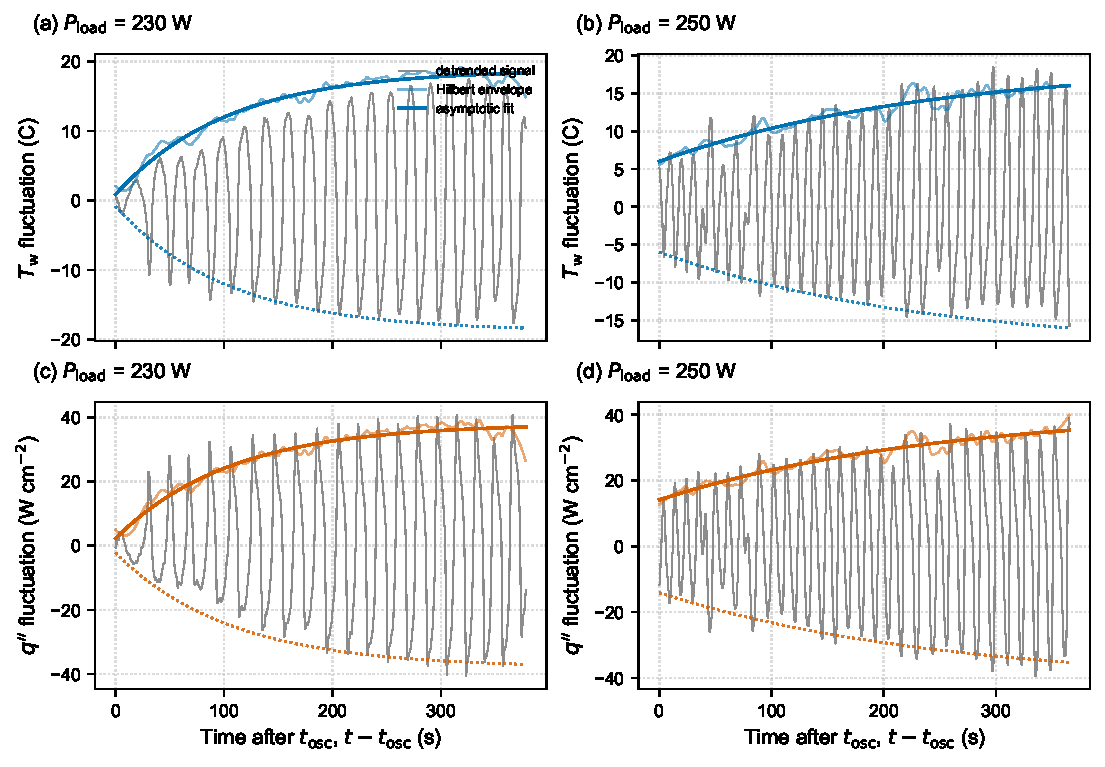
\includegraphics[width=\linewidth]{fig06_envelope_showcase.pdf}
  \caption{Raw detrended oscillations and envelope extraction for the developed high-power cases. Gray traces are detrended thermal signals; colored curves show the Hilbert envelope and the fitted asymptotic envelope. The negative fitted envelope is shown as a dotted guide to visualize the oscillation amplitude.}
  \label{fig:6}
\end{figure}

\begin{figure}[H]
  \centering
  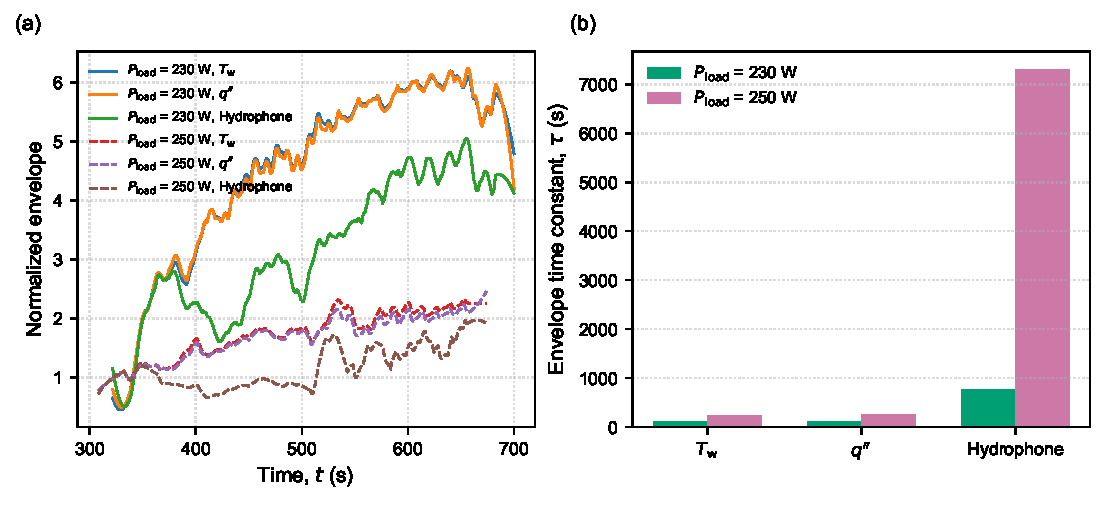
\includegraphics[width=\linewidth]{fig07_envelope_growth.pdf}
  \caption{Oscillation-envelope growth and saturation metrics for the developed high-power cases. Normalized envelopes show the different thermal and acoustic growth behavior, while the bar chart compares fitted time constants.}
  \label{fig:7}
\end{figure}

\subsection{Representative video frames and a storage-release model explain the oscillatory mechanism}

The high-speed video provides a visual basis for interpreting the low-frequency acoustic and thermal oscillations. The oscillation is not a uniform emission of small bubbles. Instead, the developed high-power cases show intervals with fewer visible microbubbles followed by intervals with dense microbubble release above the heated surface. Representative frames were selected from the MP4 videos using a frame-screening metric based on visual plume activity and annotated with the corresponding hydrophone-power percentile in the generated analysis history. The metric is computed in a fixed central plume region of interest as a weighted sum of edge density, grayscale texture, and dark-pixel fraction; it is intended only to rank frames for reproducible selection. The screening currently samples every 5 s over the oscillatory interval, giving 64 screened frames from 321.6 to 636.6 s in Case C and 66 screened frames from 308.0 to 633.0 s in Case D. In Case C, the lower-activity representative frame has a visual metric of 0.189 and coincides with the 37th percentile of hydrophone band-power proxy, while the higher-activity representative frame has a visual metric of 0.195 and coincides with the 72nd percentile. In Case D, the corresponding visual metrics are 0.187 at the 55th hydrophone-power percentile and 0.192 at the 89th percentile. Across the screened intervals, the visual metric ranges from 0.188 to 0.195 in Case C and from 0.186 to 0.192 in Case D, while the hydrophone-power percentile spans approximately 34-99\% and 42-99\%, respectively. These small metric differences are not interpreted as bubble-volume measurements. They support the frame selection and show that the many-bubble examples are tied to elevated acoustic-proxy states. The frames therefore support, rather than prove by themselves, a storage-and-release interpretation: vapor accumulates or reorganizes near the wall, the near-wall vapor/liquid system reaches a release condition, and a burst of microbubbles is emitted into the subcooled liquid.

This interpretation also provides a plausible explanation for why the reconstructed transient wall heat flux can exceed the nominal load-based heat-flux scale during the oscillatory region. The electrical input is approximately steady, but the wall/vapor/liquid system is not in instantaneous steady state. During the storage part of the cycle, energy is retained in the heated solid, vapor structure, and adjacent superheated liquid. During release, collapse, rewetting, and microbubble ejection discharge part of that stored energy over a shorter time scale. Because the present $q''$ is reconstructed from embedded thermocouple gradients, this overshoot should be interpreted as a filtered transient wall heat-flux estimate rather than direct calorimetric proof that cycle-averaged heat removal exceeds electrical input. The manuscript therefore treats the overshoot as supporting evidence for a storage-release mechanism, not as a stand-alone energy-balance measurement. In a local transient energy balance,

\begin{equation}
q''_{\mathrm{out}} = q''_{\mathrm{in}} - \frac{\mathrm{d}E_{\mathrm{stored}}}{\mathrm{d}t} - q''_{\mathrm{loss}} .
\label{eq:energy-balance}
\end{equation}

so an instantaneous local \texttt{q''\_out} estimate can exceed \texttt{q''\_in} whenever \path{dE_stored/dt} is negative and the stored energy is being released. The capacitor analogy is therefore useful, provided it is not interpreted as a literal electrical circuit. The next quantitative step is to close this energy balance over multiple oscillation cycles using the measured solid temperature field, heat losses, and time-resolved boiling images.

The same physical picture motivates a reduced-order storage-release oscillator. The model treats the near-wall vapor/thermal state as an effective capacitance, $C_{\mathrm{eff}}$, charged by the imposed heat input. Vapor-film motion, liquid inertia, and collapse/replenishment are represented by an inertial coordinate, $L_{\mathrm{eff}}$, with damping and nonlinear feedback. In nondimensional form, the conceptual model can be written as

\begin{equation}
\begin{aligned}
C_{\mathrm{eff}}\frac{\mathrm{d}\Theta}{\mathrm{d}t} &= q''_{\mathrm{in}} - q''_{\mathrm{release}}(\Theta,\xi) - q''_{\mathrm{loss}}, \\
L_{\mathrm{eff}}\frac{\mathrm{d}^2\xi}{\mathrm{d}t^2} + R_{\mathrm{eff}}\frac{\mathrm{d}\xi}{\mathrm{d}t} + K_{\mathrm{eff}}\xi &= F(\Theta,\xi), \\
q''_{\mathrm{release}} &= H(\Theta-\Theta_c)\Phi\left(\xi,\frac{\mathrm{d}\xi}{\mathrm{d}t}\right) .
\end{aligned}
\label{eq:storage-release}
\end{equation}

where $\Theta$ is a stored thermal/vapor energy state, $\xi$ is an effective vapor-film or release coordinate, $H$ is a threshold-like activation, and $\Phi$ represents nonlinear release. Figure 8 tests the most limited quantitative consequence of this model: a finite-amplitude storage-release oscillation should reproduce the measured slow period and the measured envelope growth over the sustained interval. The plotted surrogate therefore uses the fitted envelope from Figure 6 and identifies the dominant oscillation frequency by least-squares fitting a sinusoidal release coordinate to the detrended $T_w$ and $q''$ records. This is not a full parameter identification of $C_{\mathrm{eff}}$, $L_{\mathrm{eff}}$, $R_{\mathrm{eff}}$, or vapor-film geometry, but it is stronger than an unfitted sketch because the predicted oscillations are constrained by the measured amplitude growth and phase.

The model is helpful because it separates three time scales. The kHz-scale acoustic content comes from local collapse and sound generation. The 0.05-0.08 Hz oscillation comes from repeated storage and release of the MEB state. The envelope-growth time constant, reported in Table 4, describes how the oscillatory state strengthens after the first sustained peak. This hierarchy of time scales is consistent with prior visual and acoustic MEB studies, but the present dataset connects it to synchronized wall-temperature, heat-flux, hydrophone, AE, and high-speed-video observations.

\begin{figure}[H]
  \centering
  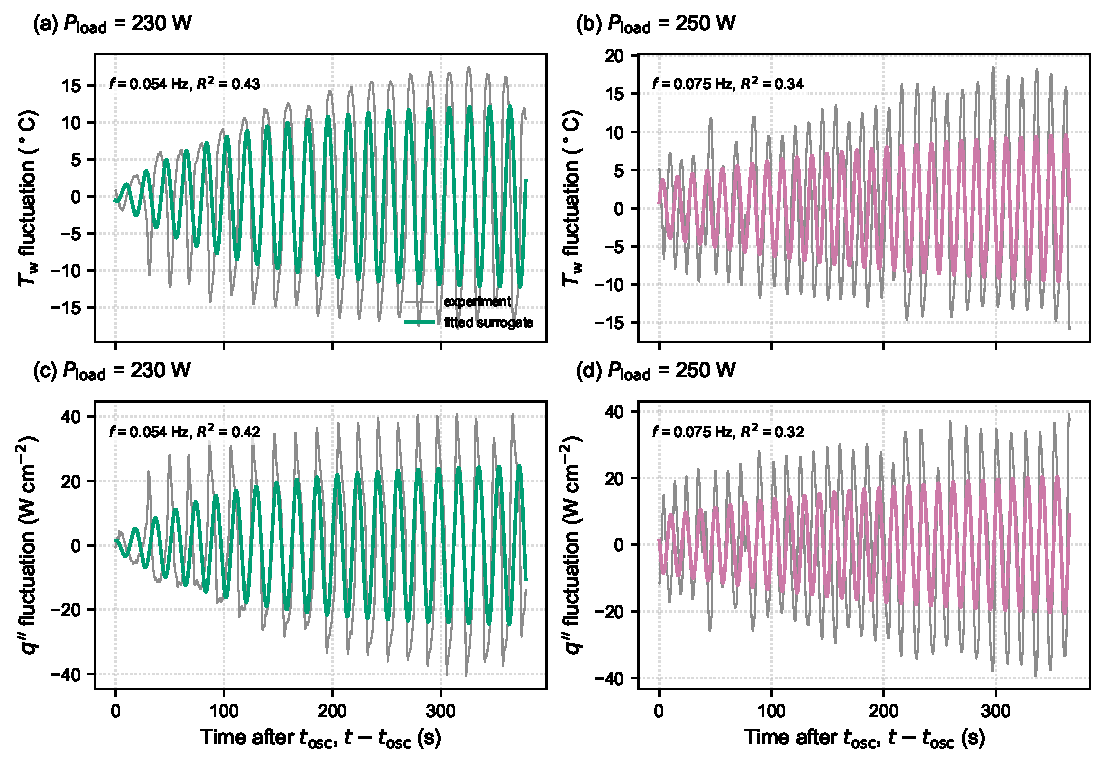
\includegraphics[width=\linewidth]{fig08_storage_release_fit.pdf}
  \caption{Data-constrained oscillatory surrogate for the developed MEB-like regime. The fitted surrogate uses the asymptotic envelope from Fig.~\ref{fig:6} multiplied by a sinusoidal release coordinate and is compared with detrended wall-temperature and heat-flux oscillations. The fit is phenomenological and is used to test whether the proposed storage-release picture can reproduce the observed slow oscillation scale.}
  \label{fig:8}
\end{figure}

\subsection{Literature comparison positions the present dataset as a diagnostics contribution}

Figure 9 compares the present cases with the screened MEB literature compilation after adding branch-level digitized traces from the available published figures. The literature now includes boiling-curve traces digitized from Ando et al. \citep{tang_2016_transition_to_meb}, Zhu et al. \citep{zhu_2014_visualized_meb}, and Horiuchi et al. \citep{horiuchi_2021_spatial_temporal_thermal_fluid}, along with a geometry-separated open-microchannel context curve from Zhao et al. \citep{zhao_2025_open_microchannel_meb}. The plotted literature values are source-status labeled by marker shape: reported or first-pass extracted values, range endpoints used only as regime envelopes, approximate figure-digitized curve points, and present reduced data are visually separated. Dotted literature traces denote non-pool-boiling geometries that should not be collapsed into the same scaling without geometry metadata. Reported and digitized heat-flux scales range from approximately 140-320 W/cm$^2$ in reduced-pressure or microchannel contexts to 600 W/cm$^2$ or higher in high-subcooling pool-boiling MEB demonstrations and specialized configurations. The present high-power cases fall within the lower-to-middle part of this broad range.

This comparison is useful because it prevents overclaiming. The present dataset does not demonstrate record-setting MEB heat flux, and Fig. 9 is not used to fit a cross-study correlation. Its contribution is the synchronized time-resolved diagnostic view: wall-temperature extrapolation, reconstructed heat flux, hydrophone power, AE waveform response where available, characteristic frequencies, and envelope saturation are analyzed on consistent event windows. That combination is less common in the literature than boiling curves, visual snapshots, or acoustic classification alone.

The upgraded comparison changes the interpretation in two ways. First, the present data are no longer being compared only with isolated literature points; the digitized traces show the path by which several published experiments approach MEB-relevant high heat flux. The present higher-power cases overlap the lower part of the published pool-boiling MEB envelope, whereas Ando et al. and Zhu et al. reach substantially higher heat flux at larger wall superheats and stronger subcooling. Second, the curve shapes reinforce why metadata matter. Horiuchi et al.'s transient pseudo-boiling curves contain large path excursions because the heat flux is reconstructed during nonsteady thermocouple response; Zhao et al.'s microchannel curves reach comparable heat-flux scales at different wall-superheat ranges because flow confinement and inlet conditions are fundamentally different from pool boiling. The literature comparison therefore supports the paper's positioning: the new contribution is not a record heat flux, but synchronized event-resolved thermal, hydrophone, AE, and visual diagnostics in a pressure-controlled pool-boiling experiment.

The remaining extraction task is narrower and better defined than before. Before using literature data for quantitative cross-study scaling, the approximate manual digitizations added here should be repeated with calibrated axes, branch labels, and source-specific uncertainty. Heating and cooling branches should be separated where published; onset points should be tied to the authors' stated MEB criteria rather than inferred only from curve shape. For heat-transfer comparison, the key quantities are MEB onset wall superheat, heat flux at onset, heat flux during stable MEB, pressure, subcooling, heater diameter or area, surface material, surface preparation, and confinement. For acoustic comparison, the key quantities are sensor type, sensor placement, bandwidth, sampling rate, frequency-definition type, spectral peak, and whether the frequency describes bubble oscillation, sound pressure, pressure fluctuation, or slow envelope modulation. Without these metadata, acoustic values from different papers can appear contradictory even when they describe different physical scales. Table 5 summarizes the literature-compiler fields that are needed before the screening comparison can be converted into a quantitative cross-study dataset.

\begin{table}[t]
  \centering
  \caption{Literature quantities needed for a quantitative MEB comparison dataset.}
  \resizebox{\textwidth}{!}{%
  \begin{tabular}{lcc}
    \toprule
    Category & Quantities to extract & Reason for inclusion \\
    \midrule
    Operating condition & pressure, liquid subcooling, working fluid, heating protocol & controls condensation, collapse, and onset path \\
    Heater and surface & area or diameter, material, finish, coating, confinement & sets heat-spreading and vapor-structure length scales \\
    Heat-transfer result & MEB onset wall superheat, onset heat flux, stable MEB heat flux, maximum heat flux & enables comparison with present heating-only boiling curves \\
    Full boiling-curve trace & digitized heating branch, cooling branch when reported, axis limits, symbol/line mapping & enables branch-resolved hysteresis and avoids reducing published curves to isolated points \\
    Time-resolved behavior & transition time, oscillation period, vapor-film or plume observations & distinguishes onset from developed oscillation \\
    Acoustic method & sensor type, placement, bandwidth, sampling rate, calibration state & determines whether acoustic magnitudes are comparable \\
    Frequency definition & carrier peak, bubble oscillation, pressure fluctuation, PSD centroid, slow envelope modulation & prevents mixing physically different frequency scales \\
    Source status & text-reported, digitized from figure, range endpoint, estimated from image & tracks confidence and reproducibility of extracted values \\
    \bottomrule
  \end{tabular}
  }
\end{table}

\begin{figure}[H]
  \centering
  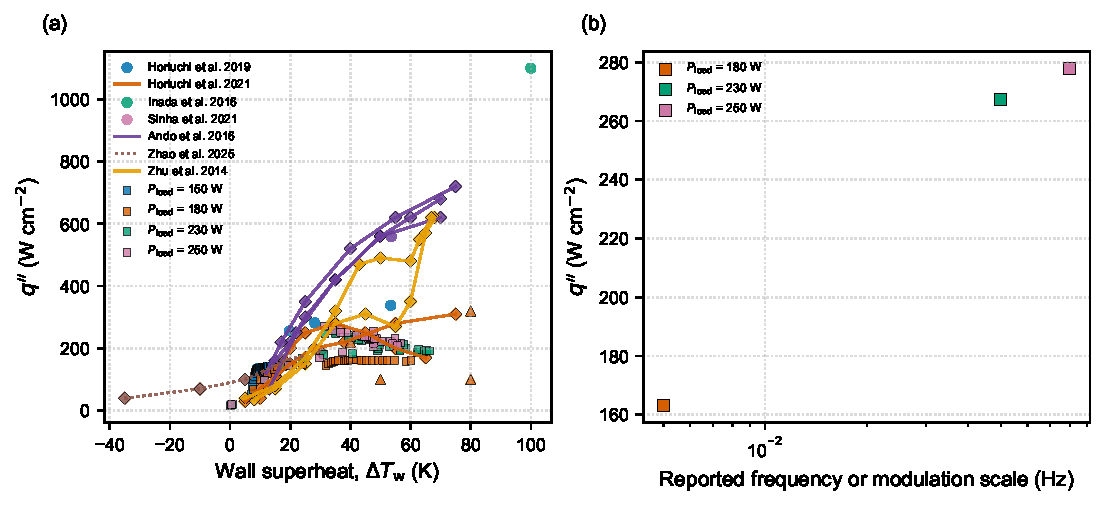
\includegraphics[width=\linewidth]{fig09_literature_context.pdf}
  \caption{Source-status-labeled literature context for the present data. The heat-transfer panel includes reported values, range endpoints, approximate figure-digitized boiling-curve traces from selected published MEB studies, and present reduced data. Dotted traces denote geometry-separated context. The signature panel separates heat-transfer quantities from acoustic or oscillatory quantities because reported frequencies may describe different physical scales.}
  \label{fig:9}
\end{figure}

\section{Limitations and Uncertainty}

The present manuscript is built on a small number of experiments. Four cases are enough to demonstrate the workflow and to identify differences between lower- and higher-power behavior, but they are not enough to establish a universal onset criterion or heat-transfer correlation. Thermal quantities are compared across all four cases. Hydrophone time histories currently cover all four cases, but MEB power-envelope frequencies are interpreted only for the developed high-power cases. AE waveform analysis is limited to the two high-power cases because those are the only cases with waveform files. Additional repeats and intermediate power levels are needed to determine whether the observed envelope time constants are repeatable and how they scale with heat load, subcooling, pressure, and surface condition.

Table 6 summarizes the calibration-limited uncertainty treatment used in this manuscript. The values are reported as expanded uncertainties with \texttt{k = 2} unless otherwise noted. Wall-temperature uncertainty is estimated as 1.72 °C from linear extrapolation of four embedded thermocouples with an assumed Type-T/DAQ standard uncertainty of 0.50 °C. Heat-flux uncertainty ranges from 8.94 to 13.09 W/cm$^2$ across the four cases because the same temperature uncertainty is propagated through different measured gradients, with a 2\% standard uncertainty assigned to copper thermal conductivity. Event-time uncertainty is 1.0 s. The characteristic-frequency resolution floor is 3.125 Hz. Hydrophone and AE band-power uncertainties remain relative because the sensors are not calibrated to absolute pressure or acoustic intensity in the present dataset; the reported relative expanded uncertainties are 46\% for hydrophone band power and 23\% for AE waveform band power. Envelope-fit parameters use a provisional 10\% standard fit-uncertainty floor, reported as 20\% expanded uncertainty. These values support within-dataset comparisons, but absolute acoustic magnitudes and final instrument-limited error bars require calibration-certificate values and bootstrap or covariance-based fit uncertainties.

\begin{table}[t]
  \centering
  \caption{Current uncertainty and quality-diagnostic status.}
  \resizebox{\textwidth}{!}{%
  \begin{tabular}{lccc}
    \toprule
    Quantity & Calibration-limited expanded uncertainty or resolution & Basis & Manuscript interpretation \\
    \midrule
    Wall temperature $T_w$ & 1.72 °C & four-thermocouple extrapolation; assumed Type-T/DAQ standard uncertainty of 0.50 °C & filtered surface-temperature estimate \\
    Heat flux $q''$ & 8.94, 9.50, 12.72, and 13.09 W/cm$^2$ for Cases A-D & Fourier-law propagation from thermocouple uncertainty plus 2\% standard uncertainty in copper thermal conductivity & filtered wall heat-flux estimate \\
    Event times & 1.0 s & wall-clock synchronization, time-bin width, and event-picking allowance & operational markers, not universal onset times \\
    Hydrophone voltage-PSD power proxy & 46\% relative & voltage PSD proxy with voltage-chain, sensitivity, and PSD-estimator terms & relative within-test acoustic activity metric, not calibrated acoustic intensity \\
    Hydrophone characteristic frequency & 3.125 Hz resolution floor & larger of spectrogram bin scale and time-window resolution & frequency descriptor tied to chosen PSD band \\
    AE waveform voltage-PSD power proxy & 23\% relative & waveform voltage PSD proxy; waveform files available only for Cases C-D & structure-path-weighted acoustic activity metric \\
    AE characteristic frequency & 3.125 Hz resolution floor & spectrogram bin-scale floor for AE waveform analysis & frequency descriptor tied to chosen AE band \\
    Envelope-fit parameters & 20\% expanded fit-uncertainty floor & provisional 10\% standard uncertainty pending bootstrap/covariance refinement & descriptive growth metrics for Cases C and D \\
    \bottomrule
  \end{tabular}
  }
\end{table}

The thermal reconstruction has its own limits. Wall temperature is extrapolated from embedded thermocouples, so high-frequency surface-temperature fluctuations are filtered by conduction through the copper block and by thermocouple response. The reconstructed heat flux should therefore be interpreted as a filtered wall heat-flux estimate rather than an instantaneous local surface heat flux. This limitation is common in conduction-based boiling measurements, but it is especially important when comparing to high-speed visual or acoustic measurements.

The acoustic measurements are reported as voltage-based proxies rather than calibrated pressure or acoustic power. Hydrophone band-integrated power has units of V$^2$ because it is derived from the measured voltage PSD. AE waveform power is similarly sensor-path dependent. Calibration, sensor frequency response, coupling, placement, and background noise must be documented before the acoustic metrics can be compared quantitatively across laboratories. The present results are strongest for within-test synchronization and relative development, not absolute acoustic intensity. The selected 0-6 kHz hydrophone integration band captures the low-kilohertz content emphasized in the present figures. The sensitivity calculation over 0-3, 0-6, and 0-10 kHz indicates that the extracted slow modulation frequency is stable for the developed cases under these nearby band choices.

The literature compilation is a screened source-status comparison rather than a definitive meta-analysis. It now contains reported-text values, range endpoints, and approximate manually digitized curve traces from selected high-priority published figures. Before using the compilation for quantitative cross-study scaling, these curves and the remaining high-priority MEB boiling curves should be redigitized with calibrated axes, branch labels, uncertainty estimates, and source-specific notes. The unpublished manuscript reviewed by the authors was used only to identify potentially relevant published references. It is not cited and does not serve as evidence in this paper.

The storage-release model is intentionally a reduced-order interpretation. The present fitted surrogate constrains the oscillation frequency and envelope with measured data, but it does not yet identify physical values of $C_{\mathrm{eff}}$, $L_{\mathrm{eff}}$, $R_{\mathrm{eff}}$, vapor-film thickness, bubble counts, or calibrated acoustic pressure. Future work can couple frame-resolved visual metrics, calibrated acoustic power, transient conduction inversion, and cycle energy balances to identify model parameters and test whether the same storage-release structure predicts repeated experiments.

\section{Conclusions}

This study develops and applies a synchronized thermal-acoustic workflow for diagnosing developed MEB-like behavior in subcooled pool boiling on a flat copper surface. The conclusions are intended as diagnostic and mechanistic findings from a four-case dataset, not as a universal MEB onset correlation. The main conclusions are as follows.

Heating-only boiling curves separate lower-power reference behavior from higher-power oscillatory behavior. Maximum reconstructed heat flux increases from 142 W/cm$^2$ in the lowest-power case to 278 W/cm$^2$ in the highest-power case. Full-history curves show hysteresis between heating and cooling, consistent with memory in the vapor/liquid structure and residual stored energy after power shutoff. Event markers further identify distinct stages of the process: the transition-associated heat-flux maximum and wall-temperature peak occur early, while the first sustained oscillation peak occurs later and defines the start of the envelope-analysis window for the developed oscillatory state.

Hydrophone measurements are available for all four cases. The lower-power cases provide acoustic references but are not interpreted as having resolved MEB modulation because they do not satisfy the combined thermal, acoustic, and visual criteria for a developed oscillatory state. The developed high-power cases show consistent hydrophone and AE slow envelope modulation. The modulation frequencies are approximately 0.05-0.055 Hz in Case C and 0.075-0.08 Hz in Case D, and the hydrophone values are unchanged across 0-3, 0-6, and 0-10 kHz integration bands in the band-sensitivity calculation. These values describe slow regime modulation, not high-frequency bubble-collapse or boiling-sound carrier frequencies. Thermal oscillation envelopes are compactly described by a first-order asymptotic growth model. Case C reaches near-saturation within the active-heating window (\texttt{tau = 103-106 s}, saturation fraction near 97\%), whereas Case D develops more slowly (\texttt{tau = 239-248 s}, saturation fraction near 77-78\% before shutoff). Hydrophone power-proxy envelopes grow but remain more intermittent than the thermal envelopes, indicating that the acoustic voltage-PSD proxy contains burst-like collapse dynamics in addition to the slow development of the MEB-like thermal oscillation.

Representative video frames show that microbubble release is temporally nonuniform. A storage-release interpretation explains this observation and provides a physical reason that reconstructed transient wall heat flux can exceed the nominal input scale during the oscillatory MEB-like regime. A data-constrained reduced-order surrogate reproduces the measured slow oscillation period and envelope form, but it is not yet a calibrated predictive model of vapor-film dynamics. The source-status-labeled literature comparison shows that the present dataset is best positioned as a multimodal diagnostics contribution rather than a record-heat-flux study. Its applied value is the synchronized connection among wall temperature, heat flux, hydrophone response, AE response, high-speed-video evidence, and envelope growth, which could support future monitoring of high-heat-flux boiling systems where optical access is limited. The reported uncertainty values support within-dataset interpretation and remain calibration-limited for absolute acoustic comparison.

\section*{Data and Code Availability}

The analysis workflow and generated figures are maintained in the BoilingLab repository. Manuscript-facing tables and publication figures are generated in the manuscript publication-analysis folder. The source-status MEB literature compilation is maintained in the separate literature compiler repository. Processed data and code are available through the repositories. Raw experimental data are stored outside the public repository in the laboratory data archive, linked internally by test metadata, and can be made available upon reasonable request subject to archive-access constraints. Restricted PDFs and publisher figures are not committed.

\section*{Declaration of Competing Interest}

The authors declare that they have no known competing financial interests or personal relationships that could have appeared to influence the work reported in this paper.

\section*{Acknowledgements}

Acknowledgements and funding information will be added before submission.

\section*{CRediT Authorship Contribution Statement}

Author contributions will be finalized before submission using the CRediT taxonomy.

\section*{Funding}

Funding information will be added before submission in the standard Elsevier format.

\bibliography{references}

\end{document}
